\def \nkois {8054}
\def \ncand {4034}
\def \newkois {738}
\def \newcand {210}
\def \completeness {85.21}
\def \reliability {97.14}
%For above numbers see script-playPublicData

\subsection{Summary of the Exoplanet Catalog}

The final DR25 KOI catalog, available at NExScI contains all of the planet candidates and all TCEs that did not fail due to one of the not-transit like tests (\S\ref{nottransitlikesec}). 


Some overall statistics of the DR25 KOI catalog are as follows:
\begin{itemize}
    \item \nkois{}~KOIs
    \item \ncand{}~PCs
    \item \newkois{}~new KOIs
    \item \newcand{}~PCs on new KOIs
    \item \completeness{} per cent overall completeness
    \item \reliability{} per cent overall reliability
\end{itemize}

A summary of the planet radii and period of the planet candidates available in this catalog can be seen in Figure~\ref{f:catalogPlot}. A clear excess of candidates exists for PCs with periods near to 370\,d;  with a score cut of $\approx0.7$, this excess disappears. While the disposition score provides an easy way to make an additional cut on the PC population at long periods, when discussing the catalog PCs below we are using the pure dispositions of the Robovetter unless otherwise stated. The deficit of planets with radii just below 2.0\,R$_{\oplus}$ is consistent with the study of \citet{Fulton2017} where they report a natural gap in the abundance of planets between super-Earths and sub-Neptunes by applying precise stellar parameters to a subset of the \kepler\ transiting candidates. 

The new KOIs with a disposition of PC are found at all periods. The overwhelming majority of these new PCs have MES less than 10; only 10 have MES >= 10. 

\begin{figure*}
    \centering
    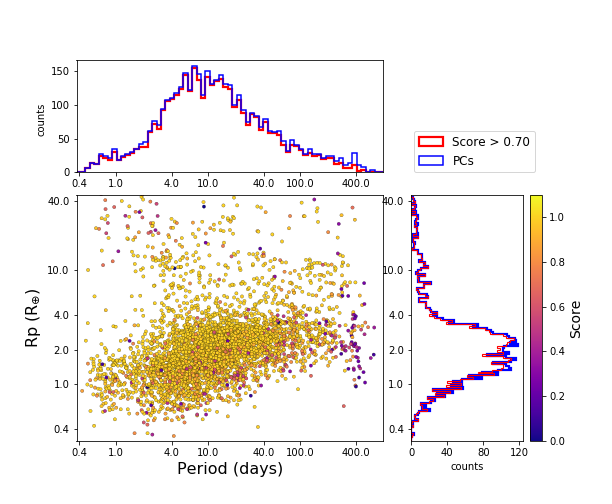
\includegraphics[width=1.1\linewidth]{fig-radiusPeriodScore-hist.png}
    \caption{DR25 planet candidates plotted as planet radius against Period with the color representing the disposition score. Those plotted in orange and yellow are those whose metrics lie near to the lest confident PCs.  The period and planet radii distributions are plotted on the top and on the left, respectively, in blue. The red line shows the distributions if you only consider those KOIs with a score greater than 0.8. }
    \label{f:catalogPlot}
\end{figure*}





\subsection{Compare Dispositions to Other Catalogs}
There are two set of \Kepler\ exoplanets that have been thoroughly vetted by hand, the confirmed exoplanets and the certified false positives.  In both of these cases, additional observations are used to fully validate the signal as either an exoplanet or a False Positive. It is worth comparing the Robovetter to these catalogs as a sanity check.  

\subsubsection{Confirmed Exoplanets}
We use the confirmed exoplanet list from NExScI\footnote{https://exoplanetarchive.ipac.caltech.edu/cgi-bin/TblView/nph-tblView?app=ExoTbls\&config=planets} on 2017-05-24.  2279 confirmed planets are in the DR25 KOI catalog.  The DR25 Robovetter fails 44 confirmed planets, less than 2 per cent. Half of these FPs are not transit-like fails, 16 are stellar eclipse fails, six are centroid offsets and one is an ephemeris match. Twelve fail due to the LPP metric, all have periods less than 50 days.  The LPP metric threshold was set to improve the reliability of the long period KOIs, an act which sacrificed some of the short period KOIs.  The reason the Robovetter failed each confirmed planet is given in the ``koi\_comment" column at NExScI (see \S\ref{s:minorflags}). 

For the vast majority of these confirmed FPs, careful inspection reveals that there is no doubt that the Robovetter is incorrect. As an example, Kepler-10b \citep[][]{Batalha2011Kepler10,Fogtmann2014Kepler10}, a rocky planet in a 0.84~days orbit, was failed due to the LPP metric. This occurred because the detrending algorithm used by the \Kepler\ pipeline significantly distorts the shape of the transit, a known problem for strong, short period signals that the LPP metric does not account for.

In some cases the Robovetter may be giving the correct disposition.  Many of the confirmed planets are actually validated \citep{Morton2016,Rowe2014}. This means that if a transit exists in the light curve and there is no evidence of a secondary event or a centroid offset then there is a high probability that the transits are caused by an exoplanet. In these cases no data additional data exists proving the existence of a planet outside of the transits observed by \Kepler. It is possible that the DR25 light curves and metrics have now revealed evidence that the periodic events are caused by noise or a binary star. For example, Kepler-367c \citep{Rowe2014}, Kepler-1507b \citep{Morton2016} and Kepler-1561b \citep{Morton2016}, (K02173.02, K3465.01 and K04169.01 respectively) were all confirmed by validation and have now failed the Robovetter because of the new ghost metric \S\ref{s:ghost}, indicating that the events are caused by a contaminating source not localized to the target star.  These validations should be reconsidered in the presence of these new validations.

\subsubsection{Certified False Positives}
We use the Certified False Positive table from NExScI on 2017-


%MUCH IS MISSING, HERE ARE SOME IDEAS:
%\begin{itemize}
%    \item [o] plot of pradius vs. period and/or pradius vs insol. flux
%    \item [o] Histogram of number of candidates of different sizes (short and long period)
%    \item [o] Discuss number of candidates compared to previous catalogs.
%    \item [o] Discuss identified EBs.
%    \item [o] From looking at distributions obvious over abundance at 370 days.
%\end{itemize}